\documentclass[shuuron]{kuee}
\usepackage[dvipdfmx]{graphicx}
\usepackage{kueecite}
\usepackage{url}

\title{チ}
\author{上}
\professor{小山田 耕二 教授}
\course{京都大学工学部}
\department{電気電子工学科 電気工学専攻}
\date{平成30年2月1日}

%%% 本文
\begin{document}
\maketitle
\tableofcontents


%%%序論
\chapter{序論}
心療において,治療者は心身症やストレスからくる身体症状をもつ来談者の治療としてカウンセリングを行う.その中で,治療者は来談者の関心つまり「対人関係上の問題」に注意を向けて引き出すということがカウンセリングの基本である\cite{zokad}.。


%%品質の定義

1.序論3
品質の定義
本論文では、「カウンセリングの品質向上への支援」を以下のように定義する。
・熟練カウンセラーからのアドバイスを含む、初心者カウンセラーのカウンセリングの質問の品質向上への支援
・クライエントの患者の認知の修正をカウンセラーが把握することへの支援
上辻は卒業研究にてここまでやったが。。。



しかし,新人治療者は「対人関係上の問題」を,質問に対する回答として来談者から引き出すのに苦戦しているという問題がある.治療者の質問内容については,大きく2種類に分けられている.YesまたはNoで答える質問,または短い言葉だけで答えられるような質問は「閉じられた質問」または「閉ざされた質問」と呼ばれている.これに対し,来談者が5W1H「いつ」「どこで」「誰が」「何を」「どのように」「どうした」で答えるような質問は「開かれた質問」と呼ばれている.熟練治療者によれば,来談者が何に問題意識を感じているかをカウンセリングで引き出すには,治療者は「閉じられた質問」よりも「開かれた質問」をしたほうがよいとされている.しかし新人治療者は「閉じられた質問」の割合が多く,来談者が何に問題意識を感じているかをカウンセリングでうまく引き出せないケースが比較的多いとされている.

このように,新人治療者は「閉じられた質問」を多く用いる傾向にあるので,熟達治療者は,新人治療者が「開かれた質問」を自由に使えるように教育したいと考えている.「対人関係上の問題」に注意を向けて引き出すということがカウンセリングの基本であるので,このように治療者の関心で来談者を誘導してしまうことはよくないとされている.そのためのチェックが可能になるものが求められている.

そこで,熟練治療者が新人治療者に指導する機会が設けられている.たとえば今回書き起こしテキストデータを使用した「心療内科における摂食障害専門ヨーガ療法グループ」事例検討会では,新人治療者に対してカウンセリングに関するアドバイスがなされている.具体的には,来談者と新人治療者とのカウンセリング内容を動画で撮影し,その動画書き起こされたカウンセリング内容のテキストデータを,熟練治療者らが読んで,議論をする,という流れである.そのため,熟練治療者達が会話の流れを文字で読むだけでは,カウンセリング内容の分析が十分に行えていなかった.新人治療者がどのような質問をして,それによって来談者からどのような回答を引き出したのか,適切な方法で可視化されることが望まれていた.

そこで本研究では,来談者と新人治療者との会話の流れを,時間軸に沿って可視化するシステムを開発した.本提案システムは熟練治療者をユーザーとして想定した.熟練治療者から新人へのカウンセリング指導において重要なことは,新人治療者が来談者にどのような質問を投げかけるかによって,新人治療者が来談者からどのような「対人関係上の問題」を引き出したかである.それが一目見てすぐにわかるようになることが,このシステムによって期待されることである.%システムをWeb上に載せることによって,同じ会話データを持っているだけで遠隔のユーザーと同様の可視化を共有することが期待される.



来談者の会話内容としては,次章で詳しく述べるどの課題領域(仕事,交友,愛)に属するのか,治療者の質問としては,内容が「開かれた質問」なのかまたは「閉じられた質問」なのかを分類表示できることが必要である.来談者からの提出した話題が,どの領域に関するものか,カウンセリングの中でその領域がどのように変わっていくかを分析していくと,そのカウンセリングプロセスがより明確になると考える.時系列に沿って見ると,最初に来談者の関心がどこにあったのか,それに対して治療者からの発話で異なった領域に話題が展開した,というような分析も可能になると考える.


本論文の構成は次の通りである.第1章は,本論文の序論である.第2章では,本論文の関連研究を挙げる.また,提案システムの開発にあたり必要になってくるカウンセリングの基礎事項について説明する.第3章では,システムの要件を整理した後,本提案システムの設計と実装について述べる.第4章では,提案システムに対する評価として,提案システムからの出力結果の内容とそれに対する考察,ユーザーからのコメントとそれに対する考察,そして本提案システムの抱えている問題点について述べる.第5章では,本論文の結論と本研究が抱える今後の課題について述べる.

%

現代社会では、多種多様なデータの膨大な量があります。具体的には、様々な会話をもとに分析テキストデータへのニーズが高まってきています。

  特に心理共同でunseling、 カウンセラーは、主にストレスの原因による物理的な症状に心身患者やクライアントとのカウンセリングを提供しています。一般的には、初心者カウンセラーは、認知特性とクライアントによる内部問題の難易度回し関心を持っています。
  初心者カウンセラーは、自分の興味に合わせて心理カウンセリングを続行する傾向があり、および周波数を使用している「クローズド・エンド型の質問(クライアントは答えることができ、 『いいえはい』または『』)」クライアントのために、人の心の中で作成された解釈を確認します。初心者カウンセラーはメイククライアントの認識こだわり答えを得ることができない
しばしば、初心者カウンセラーのはい/いいえの質問
  これとは対照的に、専門家のカウンセラーがカウンセリングの内容に関する初心者カウンセラーのための助言に教育訓練の機会を提供します。専門のカウンセラーは、そのため、初心者カウンセラーが「オープンエンドの質問(5W1Hによる質問)」を自由に使用することができます教育する必要があります。しかしながら、 なぜなら、プライバシーの問題のため、専門家は、心理カウンセリングの実際の音声データを取得することはできません。 だから、 いつも監督に、専門カウンセラーは、カウンセリングで音声表記の直接書き起こしテキストと見て、初心者カウンセラーのために誰かを教育します。
  しかし、書き起こし産物の文書 テキストデータが 心理カウンセリングにおける会話の大規模かつ複雑で、スーパーバイザは各データを参照しながら、初心者カウンセラーとクライアント間の特性との会話の状況を抽出することは非常に困難です。この問題を改善するために、我々は、会話データの可視化が有効であると思われることを検討してください。したがって、我々は、初心者カウンセラーによる各質問のためのクライアントの各回答を視覚化するための適切な方法を示すことを検討してください。
  本研究では、心理カウンセリングに会話の流れを可視化するシステムを提案し、開発しました。この提案システムでは、我々はAdlerian心理学の基礎を分類し、各カテゴリグループのためのチャートと時間の経過に沿って分布の変動を可視化表音transcriptio中含まれて、n 心理カウンセリングにいます。本稿では、システムの概要とUの結果を示します専門のカウンセラーによるSER評価。会話の流れの私達の可視化の対象ユーザーは、専門家のカウンセラーです。
   また、クライアントは、多くの場合、より多くのクライアントの「認知の補正は、」図のように心理カウンセリングに進行し、「アクションの他人の話をクライアントに自分自身を行っている」。2「彼らが行っていることを行動について話す」の割合として言います。言い換えれば、「あなた自身の行動を変えるのではなく、相手の行動を変えることに興味がある場合は、認知補正が進んでいる」[1]。したがって、我々は適切なカウンセリングの会話データから、「クライアントの行動」と「クライアントの行動を」分類し、結果を可視化することにより、クライアントの認識の変更の度合いを把握することができ、と考えました。
  上記の要求に応じて、我々は行動のどのような心理カウンセリング会話中に登場する人々の間で撮影された人間関係のチャートとを組み合わせることの方法で会話データを視覚化しようとします。


%%

会話テキストのビッグデータに溢れた時代の中で、様々な会話をもとに分析テキストデータへのニーズが高まってきている。

一方で、1991年に日本心身医学会が「心身症とは、身体疾患の中で、その発症や経過に心理社会的因子が密接に関与し、器質的ないし機能的障害が認められる病態をいう。ただし、神経症やうつ病など、他の精神障害に伴う身体症状は除外する」と定義した。そこから心身症はストレスとの深い関連が指摘された病態であると認知され、今日まで広く研究されてきた。

  そこで、心理カウンセリングにおいて、 カウンセラーは、主にストレスの原因による物理的な症状に悩む患者やクライアント(以降、クライエントと統一する)に対してカウンセリングを提供している。カウンセリングの会話記録は音声ないし動画が撮影され、後述するカウンセラー指導・事例検討の目的で役立てられているが、クライエントプライバシーの関係上実際の事例検討やカウンセラー教育の場では、それを手で書き起こした逐語録を用いることが多い。

様々な心理学の学派・セラピーが各カウンセリングに用いられているが、それらの差異にかかわらず、臨床現場でのカウンセリングの初動は、
"	インテーク面接による情報取集
"	その情報に基づいたアセスメント
"	上記のアセスメントに従った介入目標の設定とその達成方法の立案
"	それらの説明と合意をとるインフォームドコンセント
という一連の流れが含まれている。しかし初心者カウンセラーは、上記4項目の中でもまず初めの
"	インテーク面接による情報取集
でつまずいてしまうことが多い。情報収集技術には大きく分けて次の2種類の質問がある。


品質の話

Ivey,A.E. 1985のマイクロカウンセリングで示されている「開かれた質問」と「閉じられた質問」を利用する。特に、開かれた質問は情報収集を行っていくうえで特に重要で、5W1Hで質問することで、クライエント自身に答えを考え出してもらうことで、クライエント側の関心について知ることができる。                                                                            

 一般的には、初心者カウンセラーは、認知特性とクライアントによる内なる問題に対して関心を傾注することが困難になる傾向がある。

初心者カウンセラーはこの2つの質問のうち、特に閉じられた質問を必要以上に多く使ってしまう傾向があると言われている。これは
"	初心者カウンセラー自身の思い込みが先行している
"	クライエントについて十分理解できていない
ことを示している。その理由は、初心者カウンセラーが多用する閉じられた質問は、初心者カウンセラーが自身の関心でつくりあげたクライエントの像を確認しようとするために使われているからである。初心者カウンセラーが自身の関心でつくった仮説をそのまま信じることで、クライエントの症状を初心者カウンセラーがその仮説の中に閉じ込めようとしてしまう。
 それに対して、熟練カウンセラーは開かれた質問と閉じられた質問を会話の流れに応じて使い分けることで、クライエントの自身に対する洞察を支援し、クライエント自身が気づいていけるようにかかわっていく。これがカウンセラーにもできるようになるためには、カウンセラー自身が客観視を会得して、クライエント自身の関心にカウンセラーが関心を向け、クライエントが発した発言を丁寧に取り扱っていくことが可能になる必要がある。
 そこで現在、スーパーバイズ
しかし現状 
どうすれば
"	初心者カウンセラーが客観視を身に着けるために熟練したカウンセラーが行うスーパーバイズに、より客観性をもたせられるのか
"	初心者カウンセラーが客観視を身に着けるための復習に、より客観性をもたせられるか
という問題がある。
のか
そこで我々は、
"	初心者カウンセラー


  初心者カウンセラーは、自分の興味に合わせて心理カウンセリングを続行する傾向があり、カウンセラーの心の中で作成された解釈を確認する。初心者カウンセラーはクライアントの認識やこだわりに関する答えを得ることが困難になる傾向が強い。
 これはしばしば、初心者カウンセラーのはい/いいえで答えるような質問が多いことに起因するといわれている。
 以上の問題に対して、熟練したカウンセラーがカウンセリングの内容に関する初心者カウンセラーのための助言にスーパーバイズ訓練の機会を提供する。専門のカウンセラーは、そのため、初心者カウンセラーが「オープンエンドの質問(5W1Hによる質問)」を自由に使用することが可能であるスーパーバイズする必要がある。しかしながら、プライバシーの問題のため、熟練したカウンセラーは、心理カウンセリングの実際の音声データを取得することは不可能である。 そのため、 いつもスーパーバイズに、熟練したカウンセラーは、カウンセリングで音声表記の直接書き起こしテキストと見て、初心者カウンセラーをスーパーバイズする。
  しかし、書き起こしの文書テキストデータが 心理カウンセリングにおける会話の大規模かつ複雑であるにもかかわらず、スーパーバイザーである熟練したカウンセラーは各データを参照しながら、初心者カウンセラーとクライアント間の特性との会話の状況を抽出することは非常に困難である。この問題を改善するために、我々は、会話データの可視化が有効であると考える。したがって、我々は、初心者カウンセラーによる各質問のためのクライアントの各回答を可視化するための適切な方法を検討する。
  本研究では、心理カウンセリングに会話の流れを可視化するシステムを提案し、開発した。本稿では、システムの概要とUの結果を示す専門のカウンセラーによるSER評価。会話の流れの私達の可視化の対象ユーザーは、熟練したのカウンセラーである。
今回取り扱うテキストデータに記載されているカウンセリングはヨーガ療法を用いている。ヨーガ療法における病理論は、約2800年前に記されたとされる「タイッティリーヤ・ウパニシャッド」に記されている、人間を五層に分けて考える「人間五臓説」にもとづいている(p5木村先生2011)P6マンジュナートは、変化する無常なるものを普遍的なものと錯覚する「理智の誤り」、すなわち「認知の誤り」(これ以降、本論文では「認知」と統一して記す)を基準として、病気について
"	「認知の誤り」から生じない感染症や外傷などの病気
"	「認知の誤り」から生じる心身病などの病気
の2つにわけている。後者は現代心身医学のストレス認知的評価説(Lazarus, Folkman 1984)とほぼ一致してると言える(ヨーガ療法だるしゃなp7)
   また、クライアントは、多くの場合、より多くのクライアントの「認知の修正は、」図のように心理カウンセリングに進行し、「アクションの他人の話をクライアントに自分自身を行っている」。2「彼らが行っていることを行動について話す」の割合として言いる。言い換えれば、「あなた自身の行動を変えるのではなく、相手の行動を変えることに興味がある場合は、認知修正が進んでいる」[1]。したがって、我々は適切なカウンセリングの会話データから、「クライアントの行動」と「クライアントの行動を」分類し、結果を可視化することにより、クライアントの認識の変更の度合いを把握することができ、と考えた。
  上記の要求に応じて、我々は行動のどのような心理カウンセリング会話中に登場する人々の間で撮影された人間関係のチャートとを組み合わせることの方法で会話データの可視化を試みた。

 

%%%関連研究
\chapter{関連研究}
\section{結論}

本研究では,時間軸に沿った可視化によって,来談者と治療者の会話の流れを可視化するWebシステムを開発した.熟練治療者から新人へのカウンセリング指導において,どのような質問を新人治療者が来談者に投げかけるかによって,新人治療者が来談者からどのような「対人関係上の問題」に関する回答を引き出せたかが重要である.それが一目見てわかるようになったことが,本システムにて実現されたことであると考える.特にこの実現について寄与するものであると筆者が考えるのは,縦棒同士の間隔が等間隔であるグラフデザインよりも,縦棒同士の間隔の来談者の発言の文字数に比例するグラフデザインである.

しかし前章で述べたとおり,本システムのWeb上での描画所要時間は今後検証しなければならない.新人治療者を指導する目的で本システムを実用化するには,まだまだ視覚的表現やユーザーインタラクションについて議論すべき課題が残されている.次節で今後の課題についてまとめる.


%本提案システムのユーザーとして想定している熟練治療者からは「この研究が進んでいくことによって,心理臨床におけるスーパーヴィジョンにおいて,客観性にもとづく指導が可能になって
%いけることを願っております.こういう着想はありませんでしたので,大変期待
%しているところです」
%という本研究への評価を得た.


\section{今後の課題}

本研究で得られたことを踏まえて,今後検討するべき課題を簡単にまとめる.

\begin{itemize}
\item 具体的な描画所要時間の検証
\item 熟練治療者達の間でカウンセリング内容の共有が効果的に行えるようになるかの検証
\item 会話の流れの可視化に関する,他のグラフ描画方法との比較
\item 本提案システムの縦軸や横軸のスケールの取り方
\item 縦棒の上に発言番号を振ること「自己」と「スピリチュアル」のグループの追加
\item ブルーライトカットのディスプレイなどを使用しているユーザーが色を見分けにくいなどの理由から,本提案システム全体の配色面に関しての改善
\item ユーザー側で最初から最後まで簡単に可視化を行うために,カウンセリングを書き起こしたテキストデータを自動で本システムの入力データフォーマットとなる会話データに変換する機能の搭載
\item 本システムのユーザーの治療者に,入力する書き起こしテキストデータの文章量が多いと積み重ね折れ線グラフの縦棒が密集してしまう問題を解決するために,全体の積み重ね折れ線グラフから一部分を抜き出して描画するズーム機能
\item ユーザーから見た本提案システムの視覚的表現やユーザーインタラクションについての定量的な評価
\end{itemize}

新人治療者を指導する目的で本システムを実用化するために,以上の今後の課題について取り組むことが求められる.


%%


%%各論文について倍増

  の会話の関連する視覚化のいくつかの作品があります。この章では、我々は、関連する作業を説明し、我々の研究の位置を明らかにしました。本研究では、時系列に沿って視覚化方法は、テキストデータを扱う上で重要であると考えています 心理カウンセリングでの会話の流れに。


\section{会話の可視化に関する先行研究}

まず、会話を可視化している先行研究について述べ、それらの先行研究に対しての本研究の位置づけについて説明を行う。会話テキストのビッグデータに溢れた時代の中で、様々な会話をもとに分析テキストデータへのニーズが高まってきている。

Heliangは、Webベースの心理カウンセリングシステム[2]で折れ線グラフと3次元の螺旋構造を持つクライアントのトピックを可視化しました。しかし、私たちの研究では、ビューの時点で、初心者カウンセラーとクライアントの一対一の会話の流れの可視化と呼ばれる、両方で各発話内容を組み合わせることにより、可視化することが重要です。
  エリックと技術の二種類[3]で割ったトピックの時間分布のための頂部および底部の非対称層折れ線グラフにより可視化他人。私たちの研究では、上部と下部の非対称性の折れ線グラフで絵を描くための可視化技術は、クライアントによって各発話や初心者カウンセラーについて有用であることを考えます。しかし、心理カウンセリングの会話の流れを可視化するために、初心者カウンセラーによる質問に対するクライアントのどのような応答を聞くことが重要です。
  伊藤は、3次元[4]に、ブログのユーザーの興味深いトピックの時系列推移を可視化することができ、システムを開発しました。私たちの研究では、クライアントによる発話の情報は、時系列、文章のグループ、および文の数によって3次元データから構成されています。他の手で、初心者カウンセラーによって発話の情報を時系列と質問タイプによって2次元データです。しかし、我々はクライアントと初心者カウンセラーとの会話の流れが色分けして2次元のグラフで可視化することができると考えました。
   EL-Assady [5]は、スピーカからカテゴリ約トーク量を意味するサイズ文字円、トークカテゴリ円チャートと円とスピーカーパターンを分析するための視覚的な分析手法を開発しました。彼らはあなたが話題にしているサークルによって会話を表現します。
しかし、カウンセラーとクライアントのトピック分類が一緒でない限り、彼らの視覚化を使用することはできませんので、我々は彼らの視覚化からの質問と回答の間の関係を知ることができません。
  A.タットは、[6]オーディオの可視化を使用し、我々は行動を行動履歴の追加で拡張する方法を示すためにしよう

 これらのパターンの中から、トニー・バーグストロームは、[7]話し手の感情を推測することができますし、どのように彼/彼女が会話中に別のスピーカーに接続されています。しかし、A. Tatおよびトニーは、自然言語の手順を使用して、会話のコンテンツカテゴリを視覚化していないので、我々は彼らの視覚化からの質問と回答の間の関係を知ることができません。
  本研究では、このような問題は心理カウンセリングで初心者カウンセラーによってクライアントから引き出すことができる方法として、これらの発話に対応することが重要です。したがって、我々はクライアントと初心者のカウンセラーによって発話の各情報をことが望ましいと考えました コンパクトシングルチャートで視覚化する。
  ヴァンハム[8]ら。高速で文章を分析し、そのようなユーザによって指定された「BのA」および「AおよびB」との関係を有向グラフで表現されます。接続原因が入力されたテキストデータに現れたときしかし、彼らのシステムから、我々はこれらの言葉が接続されている理由を知っているとすることはできません。
  Tanakaら。 [9]効率的に話の内容をリコールインタフェースを開発しました。しかし、彼らは文字ではありませんものを含め、頻繁キーワードを可視化します。また、彼らはそれがどのようなシーンにあった、方向性、人間関係のどのような種類の部分的な可視化を行っていません。

%%

会話の可視化に関していくつかの先行研究がある。本章では、関連する研究を説明し、我々の研究の位置づけについて説明する。本研究では、時系列に沿って可視化方法は、心理カウンセリングでの会話の流れテキストデータを扱う上で重要であると考えている。
Heliang[2]は、Webベースの心理カウンセリングシステムで折れ線グラフと3次元の螺旋構造を用いてクライアントのトピックを可視化した。彼らの研究では,このような多種・多様な心理データを3D グラフで可視化する手法が提案されている.本3D グラフ表示はProcessing プロジェクトを用いて螺旋形状の表示を実
現する.また螺旋全体を回転させることで,全体的な傾向や特徴を視覚的に把握することが可能となっている
一年間を通じてどのような時期(季節,月)に相談量が多くなっているか,そしてその相
談内容の詳細も同時に容易に把握することが可能となっている.
しかし、我々の研究では、ビューの時点で、初心者カウンセラーとクライアントの一対一の会話の流れの可視化と呼ばれる、両方で各発話内容を組み合わせることにより、可視化することが重要である。
 エリックと技術の二種類[3]で割ったトピックの時間分布のための頂部および底部の非対称層折れ線グラフにより可視化他人。我々の研究では、上部と下部の非対称性の折れ線グラフで絵を描くための可視化技術は、クライアントによって各発話や初心者カウンセラーについて有用であると考える。しかし、心理カウンセリングの会話の流れを可視化するために、初心者カウンセラーによる質問に対するクライアントのどのような応答を聞くことが重要である。
 伊藤は、3次元[4]座標上に、ブログのユーザーの興味深いトピックの時系列推移を可視化することができ、システムを開発した。我々の研究では、クライアントによる発話の情報は、時系列、文章のグループ、および文の数によって3次元データから構成されている。他の手で、初心者カウンセラーによって発話の情報を時系列と質問タイプによって2次元データである。しかし、我々はクライアントと初心者カウンセラーとの会話の流れが色分けして2次元のグラフで可視化することが可能であると考えた。
  EL-Assady [5]は、カテゴリ別にトーク量を意味する円、トークカテゴリを表す円形のチャートを用いて、話者がどのカテゴリのことをしゃべっているかを表す視覚的な分析手法を開発した。彼らはあなたが話題にしているサークルによって会話を表現した。多人数会話の話者行動パターンを分析するための新しい視覚的分析手法として彼らは、会話の主題景観全体にわたる話し手の動きを追跡するためにトピック空間ビューを提案した。彼らのツールは、スピーチの相互作用や行動パターンに関する仮説を生成し、証明するために、政治学者が会話を探るのを支援することを目的としている。関連するテキストの特徴を抽象化するために、スピーカーの一般的な動作や相互作用、時間の経過に伴うインタラクティブな安定した視覚化を探索し、スピーカーの選択に関する詳細な分析を行うためのアニメーション表示を提供している。視覚的沈降法のメタファーを使用することにより、分析者は過去のすべてのスピーカーターンの概要を保持しながら、時間の経過とともに会話の流れの微妙な変化を追跡することができるようになっている。しかし、カウンセラーとクライアントのトピック分類が一緒でない限り、彼らの可視化を使用することは不可能であるので、我々は彼らの可視化方法からの質問と回答の間の関係を知ることが不可能であると考えている。
 A.タットは、[6]オーディオの可視化を使用し、我々は行動を行動履歴の追加で拡張する方法を示すためにしようとした。

 トニー・バーグストロームの可視化は、[7]話し手の感情を推測することが可能で、どのように彼/彼女が会話中に別の話者に接続されている。しかし、A. Tatおよびトニーは、自然言語の手順を使用して、会話のコンテンツカテゴリを可視化していないので、我々は彼らの可視化からの質問と回答の間の関係を知ることが不可能である。
 本研究では、このような問題は心理カウンセリングで初心者カウンセラーによってクライアントから引き出すことが可能である方法として、これらの発話に対応することが重要である。したがって、我々はクライアントと初心者のカウンセラーによって発話の各情報をことが望ましいと考えた コンパクトなシングルチャートで可視化することを試みた。
 ヴァンハム[8]らは文章を分析し、そのようなユーザーによって指定された「BのA」および「AおよびB」との関係を有向グラフで表現した。接続詞や前置詞ベースで単語をつなげている彼らのシステムから、我々は誰が誰に対して行動したかを知ることは不可能である。
 田中ら[9]は効率的に話の内容を想起できるようなインターフェースを開発した。しかし、彼らは登場人物動詞を線でのみ結んだ無向グラフとして可視化しており、その場面は誰が誰に対して行動したかをそのグラフから把握することはできない。また、彼らの可視化では章ごとのみの可視化となっており、 彼らの可視化を用いてもカウンセラーのどの質問によってカウンセリングの会話の傾向が変わったかを把握することができない。
カウンセリングについて3.基本的な説明
 本章で、我々の提案するシステムの開発に必要なカウンセリングの基本的な事項を説明する。Adlerian心理学が提案システム今回の使用データとして扱われるヨガの治療に採用されている。
アドラー心理学は、認知行動療法のパイオニアとしてみなされている。あなたがやっていることは、認知の修正であり、同様のアプローチがとられている。アドラー心理学は、オーストリアの精神科医アルフレッド・アドラー(A.アドラー)とその後継[10]によって開発された心理学の理論、思考及び処理技術のシステムである。認知行動療法はそこに来て、実験システムおよび臨床システムはかなり現代までの大まかな流れであると言われている、一緒に参加している。アドラーは、人生のすべての問題は、3つの主要なタスクに分類することが可能である」と述べ、それは、仲間の仕事、仕事のタスク、愛と家族の課題である[11] 生命タスクでAdlerian心理学、 の関係から、表のように永久的な、運命1.:質問者のための親和性、研究タスク:非常任人間関係、友情のタスク:持続性が、運命をやっていない人間関係、愛と家族の仕事。人間関係の問題を取得するのに役立ちる。「任意」(人間関係についての発言をしない)分類理にかなっている。人間関係の物語の中で3つのカテゴリで、それらにあまり動かない人と判断することが可能であるカウンセリングは、より深く、患者から悪い感情の原因を導き出すことが可能である。臨床的観点から臨床的に三つに任意の人間の問題を分類することが非常に有効であるといわれている。
我々の提案の会話の流れの可視化の前手順を 上記分類方法に基づいている。本研究では、時間軸に沿って可視化は、との会話の流れを可視化 クライアント とカウンセラーし、会話の流れが開発したカウンセラーのWebシステムによって発行された質問によってどのように変化するかを明確にしている。
一方、クライアントの認知修正の分析は、何らかの形でのように述べた行動クライアントのカテゴリを使用 図。2 動作は、クライアントの周りの人々が行っていたものが挙げられる。 鎌田は [12]、 カウンセラーの行動や感情を重要な役割は、クライアントが自己決意と自己責任を取ると不当に他人に介入することなく、他者との協力関係を形成することが可能であるようにクライアントを奨励することである。そのため、不当に他人の行動や感情に介入することなく、クライアント自身の行動や感情を見つけることが重要である。
提案した可視化システムの4前の手順
 この章で、我々は詳細に専門のカウンセラーと提案システムの設計と実装からのコメントに基づいて可視化システムを開発するための要件について説明する。

\section{カウンセリングの可視化に関する先行研究}

\section{人間関係図の可視化に関する先行研究}

カウンセリングの4.1基本的事項

\section{カウンセリングの4.1基本的事項}
4.1.1カウンセラースーパーバイズ

 臨床的観点からは、三つのカテゴリーに人間の問題を分類するために極めて有効であると考えられる。上記分類方法から、我々は次のサブセクションで提案されたシステム、設計および実装するための要件のextrbehaviorを説明する。
4.1.2クライアントの分析は
 カウンセリングで、「自分の行動を変えるのではなく、相手の行動を変えることに興味がある人は、認知を修正するに進んでいる」と言われている。ときに、クライアントの答え「クライアント自身の行動」ではなく答えるクライアントの認識の修正が進んでいると言われて、 『クライアントの周りの人々の行動を。』
 我々は、または「クライアント自身の行動」「クライアントの周りの人の行動」のデータを可視化することにより、クライアントの知覚の状態を確認可能であることを考えた。一方、我々は年代順に会話内容をテキストで行動の対象と述語を可視化することにより、上記のニーズを満たすことが可能であると考えた。このようなニーズに応えて、我々は行動の対象とオブジェクトの情報を含む人間関係チャートの時系列を可視化してきた。



%%%本提案システム
\chapter{会話の流れ可視化システム}





第1章で述べた仮説のうち、〜〜を検証するために、我々は会話の流れを可視化するシステムを開発した。本章では、本稿で述べる提案システムの1つである会話の流れ可視化システムの開発、および有効性の検証について述べる。
\section{目的}

本章では,ユーザーである熟練治療者からのコメントをもとにした提案システム要件抽出,および本提案システムの設計や実装について詳しく述べる.なお本システムでは,来談者または治療者の1発言を,話者の交代によって判断するものとする.つまり,来談者の1発言は,治療者が喋り終わって来談者が喋り始めてから,来談者が喋り終わって治療者が喋り始めるまでである.また,治療者の1発言は,来談者が喋り終わってから,あるいは治療者が話を切り出し始めてから,治療者が喋り終わって来談者が喋り始めるまでである.








\section{システム要件}




まず専門家にインタビューを行い,以下に述べるシステム要件を抽出した.




本提案システムの要件は大きく2点挙げられる.1つ目の要件は,カウンセリングにおける来談者と新人治療者との会話の流れの可視化である.カウンセリングの会話の流れのテキストデータは治療者からの発話によってまったく展開が異なってくるので,実際の来談者個人の症状の分析よりも,治療者トレーニングとして利用するのに適しているからである.本提案システムは,治療者の能力向上に資する可視化分析システムに関するものとして,治療者トレーニングの客観的指標は臨床心理学領域で期待がされている.


2つ目の要件は,来談者と治療者のそれぞれの発言を分類である.来談者の発言としては,どの1文がどの課題領域(仕事,交友,愛)に属するのか,治療者の発言としては,どの発言がオープン(5W1Hを問うもの)またはクローズ(Yes/Noを問うもの)なのかを分類表示できることが必要である.
来談者からの提出した話題が,どの領域に関するものか,カウンセリン
グの中でその領域がどのように変わっていくかを分析していくと,そのカウンセ
リングプロセスがより明確になると考えられる.時系列に沿ってカウンセリングの会話の流れを見ることで,最初にク
ライエントの関心がどこにあったのか,それに対して治療者からの発話で
異なった領域に話題が展開した,というような分析も可能になると考えられる.来談者側の関心に注意を向けるということがカウンセリングの基本であるため,治療者側の関心で来談者を誘導してしまうことはよくないとされる.そのためのチェックが本システムによって可能になることが期待される.もうひとつの課題としては,新人治療者は閉じられた質問を多用するので,新人治療者が開かれた質問を自由に使えるように熟練治療者が指導する必要がある.そのチェックも本システムによって可能になることが期待される.




\subsubsection{来談者の発言に関する分類}



来談者の発言に関する分類に関しては,1発言単位ではなく1文単位で「愛」「交友」「仕事」を分類するように変更することが求められる.
たとえば,「うちの夫は仕事にいくのを嫌がって,毎朝起きてこないんです.
それを見ているだけで腹が立つんです.自分の同僚が同じように仕事に行きたが
らなくて朝起きなかったという話を聞いても,さほど腹は立ちませんが,夫がそ
うなるのは絶対に許せない」という文章について,専門家は次の通りに分類する.第1文は愛の課題,第2文は仕事の課題,第3文は愛の課題に分類する.
原文から,治療者から来談者への質問事項の分類の指標として,来談者の発言をうながして来談者自身も気づいていなかったことを認知させるのが大事であるので,それぞれの発言量の可視化の実装を盛り込むべきであるというコメントを得た.ここから得られる要件は,来談者の発言の分量に応じて,それをはさむ治療者の発言の縦棒をグラフ上で変えることであると考えた.

\subsubsection{治療者の発言に関する分類}

治療者の発言の分類について,まず治療者の発言も,次章で述べる初期分類は適当ではないことがあるので,来談者からの返答だけでなく,治療者の質問区分けも手動で修正したいというコメントを得た.
また,治療者の発言について,「開かれた質問」「閉じられた質問」だけでなく,「解釈」「相槌」「無駄話」という分類を追加してほしいというコメントを得た.
来談者の発言に関する分類とは異なり,治療者の発言に関する分類は1文単位ではなく1発言単位での分類でよいというコメントを得た.







\section{システム設計と実装}

前節では提案システムのユーザーである熟練治療者からのコメントをもとにした,提案システム要件抽出について説明した.本節では提案システムの設計と実装について説明する.本節ではその要件をみたした提案システムの設計と実装について説明する.

まず本提案システム評価で使用する入力データについて述べる.本章の提案システムにおいて,カウンセリングを書き起こしたデータを全15個に分けて使用した.以降この15個のデータをそれぞれ,会話データ1,2,3,……,15と呼ぶこととする.この本論文の実験で用いる対象データには「ヨーガ療法事例検討会」資料から引用したものである.
また,後述する初期グラフ描画がある程度有用なものかを示すために模擬会話データを1個用意した.

次に,本提案システムのアルゴリズムについて説明する.
なお,本提案システムの開発言語はJavaScriptである.
%本提案システムの構成を図\ref{fig:4_2}に示す.
また本提案システムのユースケース図を図
%\ref{fig:use_case_diagram}
に示す.
ユースケース図は,システムがどのように機能すべきか,およびその外部環境を表すUMLの図である.
UMLは,主にオブジェクト指向分析や設計のための,記法の統一がはかられた(Unified)モデリング言語(Modeling Language)である.


\begin{figure}
   \begin{center}
  %   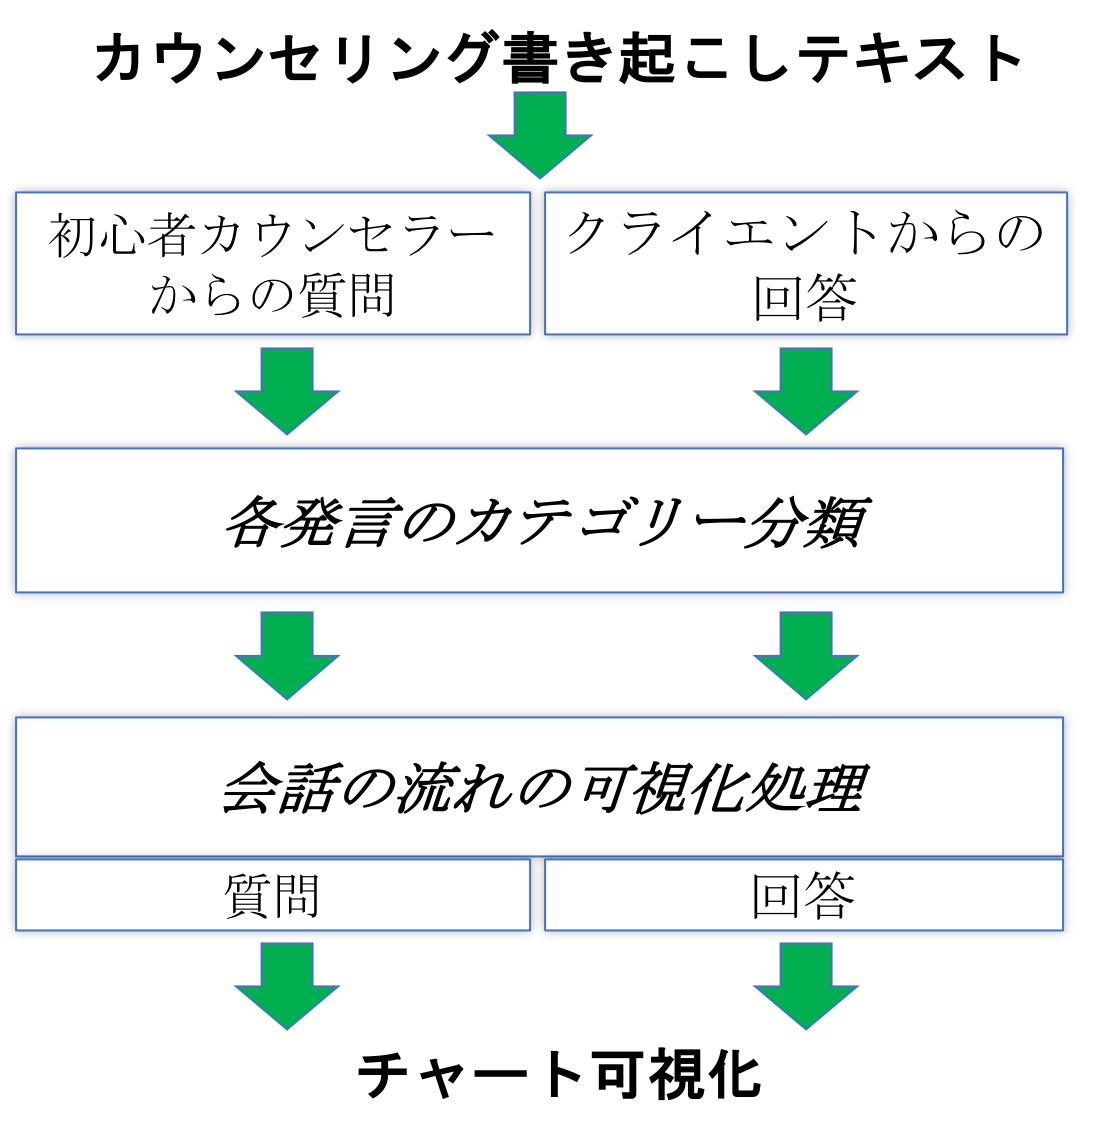
\includegraphics[width=\linewidth]{4_2.png}
   \end{center}
   \caption{提案システムの構成}
   \label{fig:4_2}
 \end{figure}

\begin{figure}
   \begin{center}
     % 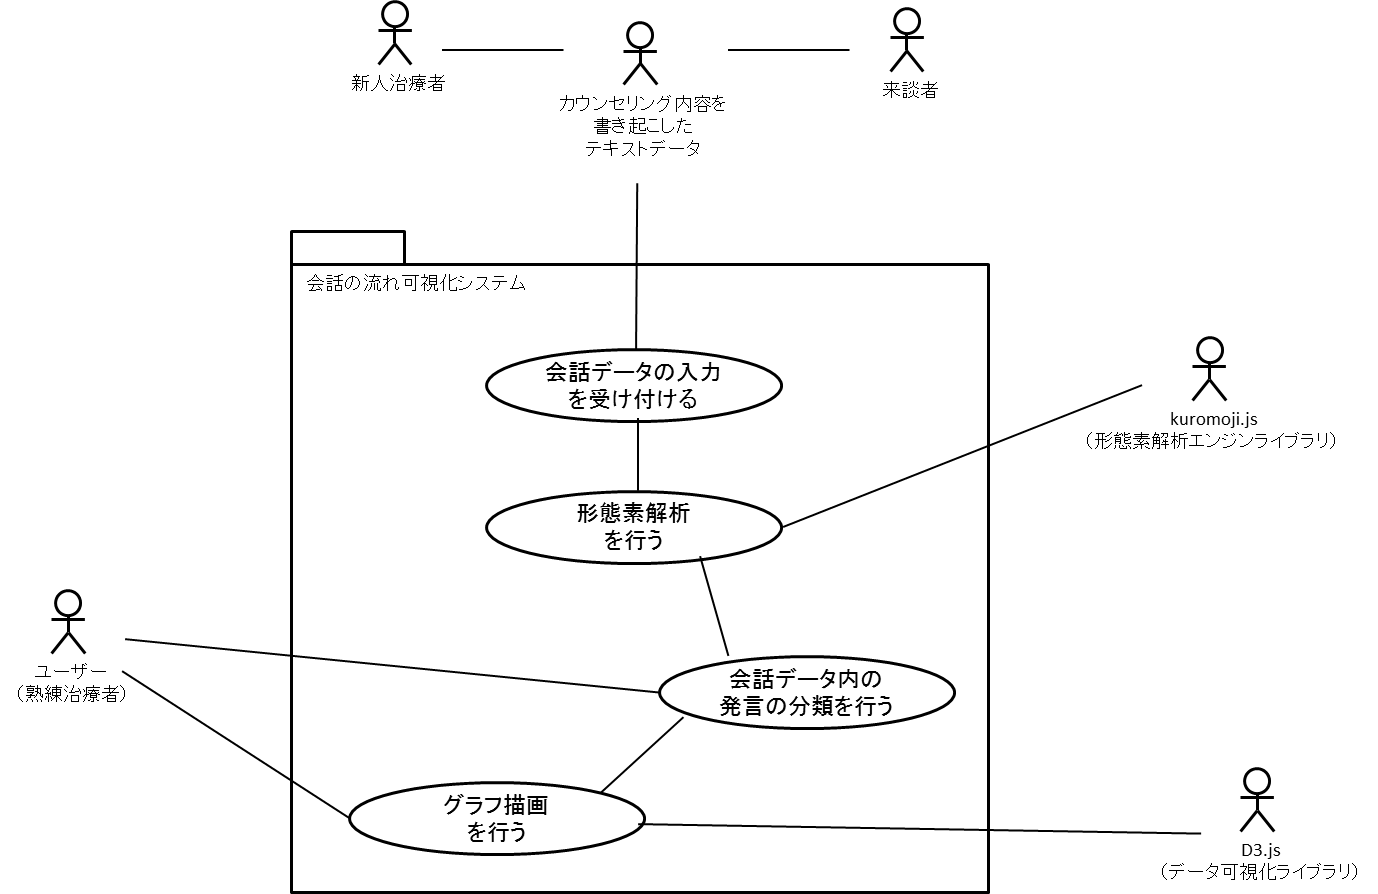
\includegraphics[width=\linewidth]{use_case_diagram.png}
   \end{center}
   \caption{提案システムのユースケース図}
   \label{fig:use_case_diagram}
 \end{figure}


まず,グラフ描画前のテキストデータ処理について述べる.アクティビティ図を図
%\ref{fig:activity}
に示す.アクティビティ図とはフローチャートに似た図で,いわゆるビジネスロジックにおける手続き的な流れやプログラムの制御フローを表すUMLの図である.
\begin{figure}
   \begin{center}
     %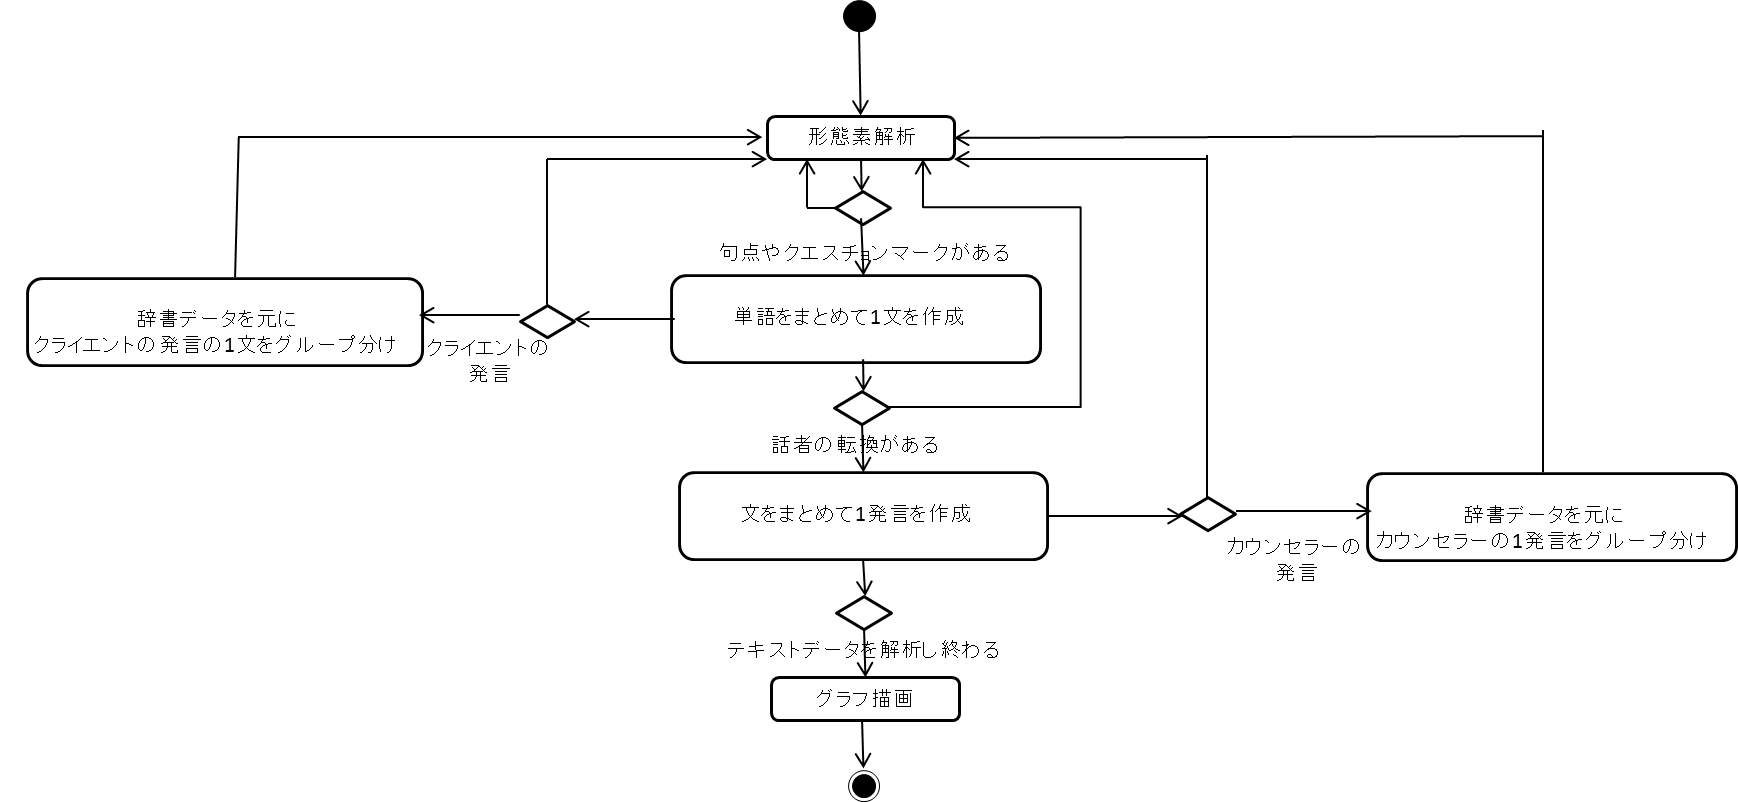
\includegraphics[width=\linewidth]{activity.png}
   \end{center}
   \caption{テキストデータ処理のアクティビティ図}
   \label{fig:activity}
\end{figure}


初めに,ブラウザ上で各テキストの会話データを読み込んで,テキストを単語ごとに区切る形態素解析を行う.会話データ読み込み前の本提案システムスクリーンショットを図
%\ref{fig:yomikomimae2}
に示す.
 \begin{figure}
   \begin{center}
     %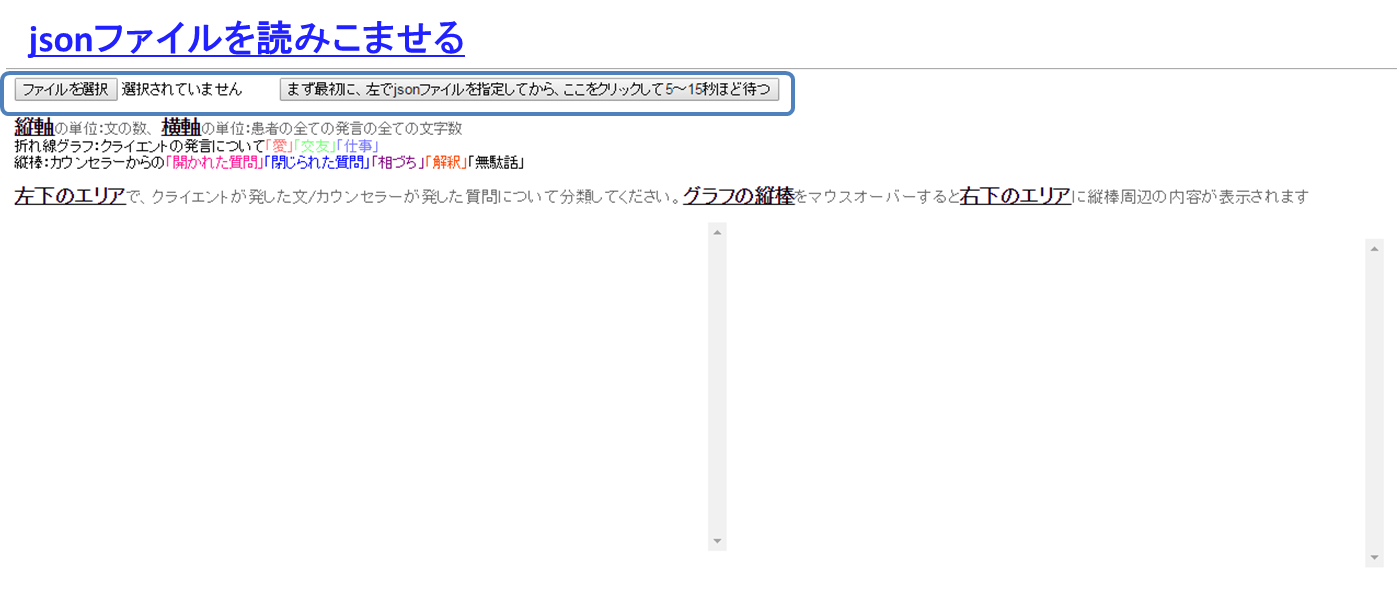
\includegraphics[width=\linewidth]{yomikomimae2.png}
   \end{center}
   \caption{会話データ読み込み前のシステムスクリーンショット}
   \label{fig:yomikomimae2}
 \end{figure}
形態素解析サブシステムには,JavaScript言語の形態素解析ライブラリであるkuromoji.js\cite{kuromojijs}を使用した.kuromoji.jsは,Javaで実装されたオープンソースの日本語形態素解析エンジンKuromoji
%\cite{kuromoji}
を,JavaScriptに移植したものである.

%\subsubsection{1文や1発言の作成と分類}
形態素解析された単語群から,句点やクエスチョンマークを終点と定義して1文ずつのテーブルをつくる.さらに,話者の切り替わりを全角コロンで定義し,全角コロンと全角コロンの間の文のグループを1発言と定義し,発言単位でテーブルをつくる.「来談者の発言においてこれを含む文はこのグループに属するだろう」という単語を,「愛」「仕事」「交友」ごとに指定しておき,発言データの文を構成する単語が指定された単語と一致する場合,この情報を図
%\ref{fig:4_2}
の発言データ分類サブシステムに引き渡し,発言データ分類の初期設定値を計算する.
%この初期選択において,今回は簡単化のため,複数のグループの可能性をもつ1文に対しては,「愛」の可能性があれば「愛」に,それ以外は「仕事」に分類するようにした.



質問内容は,前章の要件通り 5 種類に分類され,後述する縦棒アイコンの色の割り当ては次の通りである.赤色は5W1H「いつ」「どこで」「誰が」「何を」「どのように」「どうした」などで問われるような「開かれた質問」,青色はYes/Noで答えられる,あるいは一言だけで簡単答えられるような「閉じられた質問」,紫は「相槌」,オレンジは来談者の問題を治療者がどう「解釈」しているかの確認,黒は「無駄話」を表現している.第1章で述べた通り,来談者が何に問題意識を感じているかをカウンセリングで引き出すには,治療者は「閉じられた質問」よりも「開かれた質問」をしたほうがよいとされている.


治療者の1発言についても,来談者の発言の1文ごとの分類と同様に,関連する単語をあらかじめ指定しておき,必要情報を
%\ref{fig:4_2}
の発言データ分類サブシステムに引き渡し,発言データ分類の初期設定値を計算する.

ここで会話データを入力した後の治療者の初期分類状態の分類方法について説明する.今回の実際の会話データ15個のうち,治療者の発言数は398発言あったが,本システム要件の質問分類の「相槌」に含まれるべき短文に「そうですか」というフレーズが41箇所あった.富士通株式会社は質問文判定について特許
%\cite{tokkyo}
を取得しているが,富士通株式会社の特許技術において行われている「(ます)か」という文の終わり方だけで質問判定を行うだけでは,「そうですか」というフレーズも自動的に「相槌」ではなく「閉じられた質問」に分類してしまうので不適当である.

本システムにおける,会話データを入力した後の治療者の初期分類状態の分類方法を簡単に図
% \ref{fig:5_2}
に示す.
% \begin{figure}
% %\begin{landscape}
%    \begin{center}
%      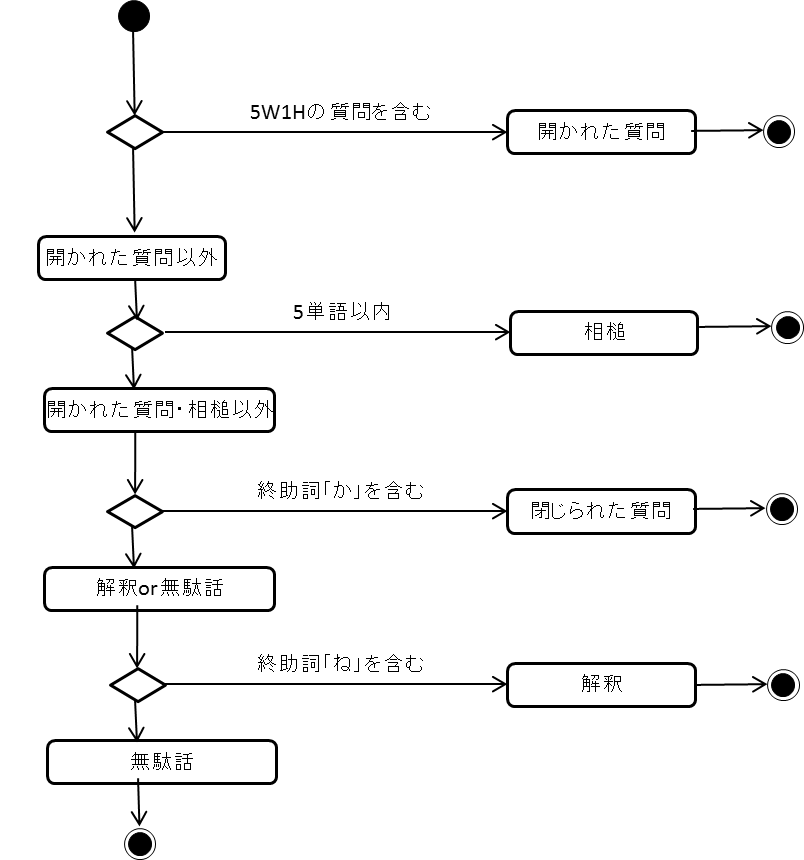
\includegraphics[width=\linewidth]{5_2.png}
%    \end{center}
%    \caption{治療者発言初期分類方法}
%    \label{fig:5_2}
% %\end{landscape}
%  \end{figure}
まず「いつ」「どこ」「何」などのいわゆる5W1Hを示す疑問詞をもつ発言を「開かれた質問」に分類する.次に残りの発言のうち,単語数が5個以下のものを「相槌」に分類する.さらに残りの発言のうち終助詞「か」を含む発言を「閉じられた質問」に分類する.今までの3つに分類されなかったものは「解釈」か「世間話」に分類されるわけだが,終助詞の「ね」を含むものを「解釈」,含まないものを「世間話」とした.

%\subsubsection{グラフ描画}
以上がグラフ描画前のテキストデータ処理である.その後,治療者からの質問形態と, 「愛」「仕事」「交友」の文のグループの時間経過に沿った分布変化を可視化する.グラフ描画の際に,会話データを発言データ可視化サブシステムに受け渡す.このサブシステムでは,データ可視化ライブラリD3.js
%\cite{bostock2012d3}
を使用した.模擬会話データを入力した際の出力結果を図
% \ref{fig:6_1}
に示す.また模擬会話データの原文と,模擬会話データ時の初期自動分類結果を表
% \ref{table:book1}
に示す.
% \begin{figure}
%    \begin{center}
%      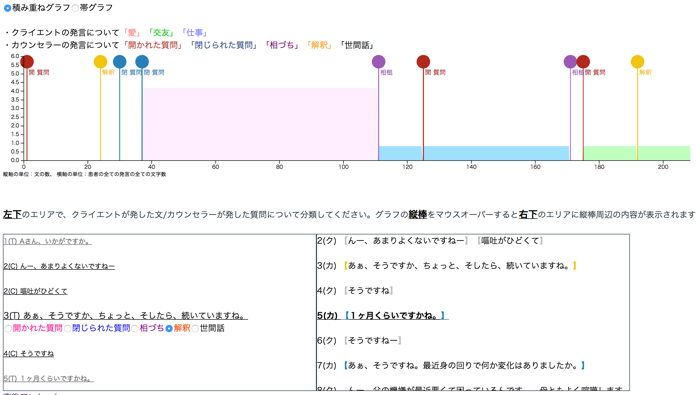
\includegraphics[width=\linewidth]{6_1.png}
%    \end{center}
%    \caption{模擬会話データでのシステム出力結果}
%    \label{fig:6_1}
%  \end{figure}
%
% \begin{table}
%    \caption{模擬会話データでの初期表示用自動分類結果}
%    \label{table:book1}
%    \begin{center}
%      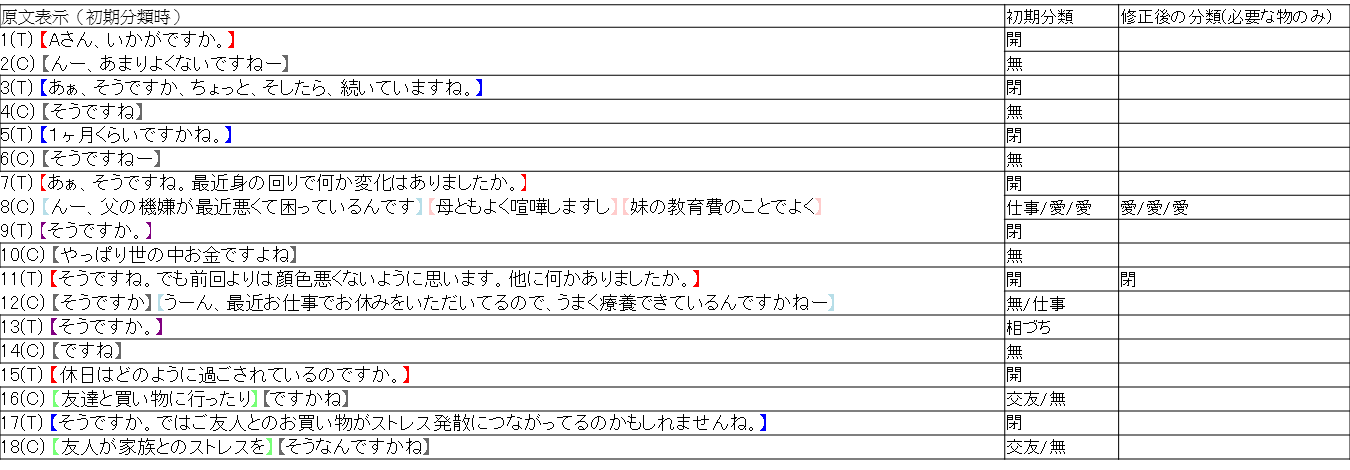
\includegraphics[width=\linewidth]{book1.png}
%    \end{center}
%  \end{table}

\subsubsection{来談者発言ビュー}
次に〜〜について用いる、クライエント発言ビューについて説明する。
図
%\ref{fig:6_1}
において,まず積み重ね折れ線グラフは来談者の1回の発言の中での,アドラー心理学の各カテゴリの分布を可視化している.ただし1回の発言は,話者の交代を発言の区切れ目とする.この積み重ね折れ線グラフにおいて薄い水色は「仕事関係」,ピンク色は「愛(恋愛・愛関係)」,薄い緑色は「交友(友人関係)」に密接に関係する単語を含む文の分布を表している.
横軸は時間軸を表現している.ただし対象データである書き起こしテキストデータからは実際の経過秒数は読み取れないので,読み込ませたデータ内における来談者の発言量の累計の文字数を横軸,つまり時間軸とした.後述する治療者の質問を表現する縦棒はこの時間軸にそって出現する.治療者と来談者の発言の入れ替わりがわかりやすいように,積み重ね折れ線グラフが来談者の発言のグループ分布をちょうど表しているのは便宜上発言部分の中央部分になっている.
縦軸は発言中の1文の数のうち,どのグループに何文入っているかという文の数を表している.

%ここで会話データを入力した後の来談者の発言の各1文の初期分類状態の分類方法について説明する.
%まず,あらかじめこちらで
%次に,各単語群を含む来談者の発言の1文をグループ分けをしていった.




\subsubsection{治療者発言ビュー}

Ericら
%\cite{taskdriven}
は,トピックモデリングによって分けたトピックの時間分布を上下の非対称積み重ね折れ線グラフによって可視化した.一方本研究では,治療者と来談者の会話において,来談者は文ごとに,治療者は発言ごとに描画を行いたい,かつ選択肢表示のためにグラフを省スペースしたいという観点から,治療者の発言を横軸より下に折れ線グラフとして描画するのではなく,来談者の発言のグループ分布を示す積み重ね折れ線グラフに重ねて縦棒として表示するようにした.こうすることによって,来談者と治療者の発言が交互に描画されるので,来談者と治療者の発言の関連性がわかりやすくなった.積み重ね折れ線グラフに重なっている縦棒は,治療者の質問内容の形態を示す.


\subsubsection{発言分類手動修正機能}
積み重ね折れ線グラフが描画された後に,グラフ左下のラジオボタンエリアにて,クライアントの発言の各1文および治療者の各1発言において,分類を変えると即時にグラフ描画に変更が適用されるようにした.
%本ラジオボタンエリアがみたした要件については,付録にて記述する.

\section{要件抽出}

%%修論からパクってくる

 この章で、我々は我々の提案するシステムの開発に必要なカウンセリングの基本的な事項を説明します。心理療法では、単一であり、すべての通信を全く学校はありません。最大の学校は、認知行動療法と言われています。しかし、Adlerian心理学が提案システム今回の使用データとして扱われるヨガの治療に採用されています。
アドラー心理学は、認知行動療法のパイオニアとしてみなされています。あなたがやっていることは、認知の修正であり、同様のアプローチがとられています。アドラー心理学は、オーストリアの精神科医アルフレッド・アドラー(A.アドラー)とその後継[10]によって開発された心理学の理論、思考及び処理技術のシステムです。認知行動療法はそこに来て、実験システムおよび臨床システムはかなり現代までの大まかな流れであると言われている、一緒に参加しています。アドラーは、人生のすべての問題は、3つの主要なタスクに分類することができる」と述べ、それは、仲間の仕事、仕事のタスク、愛と家族の課題である[11] 生命タスクでAdlerian心理学、 の関係から、表のように永久的な、運命1.:質問者のための親和性、作業タスク:非常任人間関係、友情のタスク:持続性が、運命をやっていない人間関係、愛と家族の仕事。人間関係の問題を取得するのに役立ちます。「任意」(人間関係についての発言をしない)分類理にかなっています。人間関係の物語の中で3つのカテゴリで、それらにあまり動かない人と判断することができますカウンセリングは、より深く、患者から悪い感情の原因を導き出すことができます。臨床的観点から臨床的に三つに任意の人間の問題を分類することが非常に有効であるといわれています。
私たちの提案の会話の流れの可視化の前手順を 上記分類方法に基づいています。本研究では、時間軸に沿って可視化は、との会話の流れを可視化 クライアント とカウンセラーし、会話の流れが開発したカウンセラーのWebシステムによって発行された質問によってどのように変化するかを明確にしています。

\section{開発}

%%修論からパクってくる

前節で述べた要件抽出にもとづいて、我々は会話の流れ可視化システムの開発を行った。本節では、会話の流れ可視化システムの、可視化する前の処理の部分について説明を行う。



  臨床的観点からは、三つのカテゴリーに人間の問題を分類するために極めて有効であると考えられます。上記分類方法から、我々は次のサブセクションで提案されたシステム、設計および実装するための要件のextrbehaviorを説明します。


  このセクションでは、提案システムの設計と実装について説明します。図3は、カウンセリングでの会話の流れの可視化システムの処理手順を示しています。会話の流れの可視化は)1つのカウンセリングセッションでの会話の内容を示しています。このシステムでは、可視化の前処理として、カウンセリングにおける会話のテキストデータのカテゴリ分類が実行されます。
  このシステムでは、担当者やカウンセラーからの1つのコメントは話者の変更によって判断されます。カウンセラーが話し終えるとクリニックが話すと、治療が話し始めるまで話者が、話し始めるまで、言い換えれば、話者の1から1件のコメントです。また、ずつutterancはe  、 カウンセラー話者が話し、またはカウンセラーが話し終わるまでカウンセラーが、話を引き裂く起動し、情報提供者が話し始める終了時からです。
  このシステムでは、クライアントの発話は、それぞれの文は、アドラー心理学に基づいて、タスクエリア「仕事」、「友情」と「愛と家族」に相当します。図4は、表.2のようにカウンセラーの質問の自動分類方法の流れを示し、表2に示すように、他の手で、初心者カウンセラーによって発声は5つのカテゴリに分類されています。まず、「いつ」、「どこで」、「何を」として、「5W1H」を示すinterrogatives、との声明を分類し、その上の「オープン質問」など。次に、残りの発話のうち、5つの以下の単語を有するものは、「フィードバック」として分類されます。さらに、残りの発話のうち、「KA」日本の最終的な封入粒子を含む発話が「閉質問」として分類されます。限り過去、「解釈は」日本最後のエンディングの粒子「NE」と「アイドルの話」を含むもののために含まれているとして分類されていなかったものの中に日本人が含まれないものを除外することです。
まず、提案システムは、ブラウザ上で各テキストの会話データを読み、言葉にテキストを分離するために形態素解析を行います。使用されたJavaScript言語の形態素解析ライブラリである形態素解析サブシステム、kuromoji.js [13]のために。 kuromoji.jsはJavaScriptに移植されたJava Kuromoji [14]に実装オープンソース日本語形態素解析エンジンです。
  次に、これらの文章は、このシステムに登録カテゴリーと文の各単語に対応するキーワードとのマッチングにより、各カテゴリに分類されています。しかし、このカテゴリの分類方法ではカウンセラーとクライアントによって各発話のテキストデータに適用し、分類結果の精度は、システムに登録されている単語辞書に依存し、分類のための正解率は非常に低いです。そのため、専門家のカウンセラーは、現在のシステムでは、最初の分類結果を確認し、手動で誤った分類結果を修正する必要があり、作業負担が大きいました。クライアントのそれとは違って、私はセラピストの発話の分類は、文単位が、話し手ターン単位での分類ではないというコメントを得ました。
発話データの分類後、クライアントによる発声のための初心者カウンセラーと「仕事」、「友情」と「愛と家族」に関連した文のカテゴリグループのための時系列での分配変化による質問の形式は、同じ時代に可視化しました。





\section{可視化結果}

前節では、会話の流れ可視化システムの可視化前の処理の部分の実装について説明を行った。本節では、その前処理後の可視化の処理の部分について説明を行う。


%%可視化結果をゴリゴリ説明

時系列人間関係チャートの画像を示しています。下のスライダーを動かすことによって、私たちはどのような文を時系列に沿ってどのような文に、例えば、人間関係からチャートを表示しました。また、図2に示すように、それが可能な、対応する動詞の文章を表示することによって、我々は、矢印は、図手段として、元のどのテキストを知ることができる。7. 私たちは、可視化のためD3.js [17]を用います。



\section{User Evaluationと考察}

前節までは、会話の流れ可視化システムの開発およびケーススタディについて説明を行った。本節では、会話の流れ可視化システムを用いて「」という仮説を検証するために行ったユーザ評価の目的・手法・結果・考察についてのべる。

%%ユーザエバリュエーションをゴリゴリ説明

  専門カウンセラーが、彼は「私はBが私の意志に従うことをしたい」という考えが消えていることが分かったと述べました
自己閉じタスクが増加しました。認知の補正の進行は、することができました 量変更することによって確認 矢印の(複数カウンセリングの全体図)をし、元のテキスト表示で品質を確認。 我々は、我々の提案文字チャートの可視化は、カウンセラーは見つけることができますことを検討してください のいくつかの種類がことを 、クライアントの 認知の修正作られた。
\subsection{シグマ値法}
多数の意見項目などを多変量解析で分析する際に、態度を測るものさしであるカテゴリー尺度は、本来は順序尺度なので、間隔尺度に換算して重み付ける必要がある。しかし通常は、回答ガテゴリーのコード番号を間隔尺度の得点として簡便に用いている。

通常の例の場合に対して、心理学では、カテゴリーの順序尺度を間隔尺度に換算する方法を持っている。その一つにシグマ値法(系列カテゴリー法ともいう)が存在する。シグマ値法は、意見項目の各カテゴリーに対する一連の回答率を、標準正規分布の面積と考え、面積に対応する縦座標と面積の比という間隔尺度に置き換える方法である。

標準正規分布は、元のデータを0、標準偏差1.0に換算したデータのことである。シグマ値法においては、回答カテゴリーの回答率を標準正規分布の面積と考えて、面積に対応する縦座標の比に置き換えることによって、順序尺度を間隔尺度に置き換えることが出来ている。
シグマ値法は以下の手順に従って算出される。
\begin{enumerate}
 \item 各カテゴリーの順番を下位のものから上位のものに整列させる
 \item 格カテゴリーへの度数から比率を計算する
 \item 各カテゴリーの累積の比率を算出して、下限値から上限値までを計算する。
 \item 各カテゴリーの累積の比率の最小値と最大値を標準正規分布の縦座標に置き換える
 \item シグマ値を計算する
 \item カテゴリー得点の計算を行う。
\end{enumerate}

以上のシグマ値法で換算した値を用いて、多変量解析をおこなうことによって、「悪いが1点、やや悪いが2点、……」のようなカテゴリー得点をカテゴリーの数字で代替する通例の手法よりも明快な解析結果が得られると言われている。

\subsection{原文を読むこととの比較}

\subsection{形状比較}
上辻の卒論で取り扱った形状との比較を行った。

前章で述べた会話の流れの可視化システムを,3名の熟練カウンセラーに評価者として実際に使用してもらうことで,システム評価を行った.熟練カウンセラーの平均年齢は55歳,平均臨床歴は29年であった.
まず評価者は,積み重ねグラフ,帯グラフそれぞれについて,あらかじめ表示されている可視化結果に対して,時系列に沿ってマウスカーソルを合わせることで,カウンセリングの流れを一通り確認する.その後,6段階評価によるアンケート質問に回答を行う.6段階評価のアンケートの質問項目,および各質問に対する選択肢とその配点をTable 1に示す.Table 1の各質問項目は,積み重ねグラフ,帯グラフそれぞれに対して行った.積み重ねグラフ,帯グラフについて,各質問項目に対する6段階評価の平均値の結果をFig.5に示す.Fig.5 の結果より,全ての項目において,積み重ねグラフより帯グラフの方が優れていることがわかった.

%%有意差、相関関係

さらに本評価では,以下の(1)~(5)に記す自由記述の 質問を行った.

(1)	帯グラフを見て,カウンセラーに対してどのような指導ができるでしょうか
(2)	グラフについて,その他全体的に何かご意見が  あれば,ご回答ください
(3)	このシステム全体を用いて,カウンセラーに対して指導できそうなことがあれば,ご回答ください
(4)	原文表示機能について何かご意見があれば,ご回答ください
(5)	このシステムについて,何か他に欲しい機能が  あれば,ご回答ください

質問(1)に対して

  一回のカウンセリング全体を俯瞰し大まかな カウンセリングの流れを指導
  クライエントとカウンセラーが時系列で対比 しながら見ることができるので,一回の面接での流れ,例えば,前半はクライエントに多く喋ってもらっていたのが,後半ではカウンセラーが喋っていたとか,解釈の時に発言量が多いとかが指導できるように思いました

といった回答が得られた.これより,全体を俯瞰して発言量の分布の変化を基に新人カウンセラーに対して,様々な指摘を行えることが考えられる.
質問(2)に対しては「帯グラフで,それぞれの発言内容の語数や時間が表示されれば,さらに便利かなと思いました」という回答が得られた.
質問(3)に対しては

  カウンセラーの発言のチェックとクライエントの関心に関心を向けているかのチェック」「一回のカウンセリングでカウンセラーとクライアントがどのような作業を協力して行っているのか理解を深めること,カウンセリングが成立するためにはカウンセラーとクライアントの間で相談的人間関係が構築できていることが前提となることを理解するのに役立つ
  カウンセリングがこのように可視化されることだけでも,とても有意義だ
  この結果をもとに,カウンセリングを再構築するための材料としても使える

といった回答が得られた.
質問(4)に対しては「カウンセラー,クライアントが  どこでどんな発言をしているのか確認するのに役に立つと思いました」という回答が得られた.
以上の結果から,積み重ねグラフよりも帯グラフの方が,新人カウンセラー指導に優れていると結論づけられる.また全体として,本システムが新人カウンセラーに対する指導を行うために,会話の流れが適切に可視化されていることが,複数名の熟練カウンセラーからの回答によって結論づけられると考える.
 質問(5)に対しては

  カウンセラー,クライアントの発言を音声で確認できる機能,カウンセリング中のクライアントの身体の動きの変化(カウンセリング開始から本題にはいるまで〈相談的人間関係構築がなされているかどうか確認のため〉また特にカウンセラーが解釈投与した直後のクライアントの身体の動き〈解釈投与に対してクライアントがどのような認識反射をおこなっているのかを確認するため〉)についても記されていると便利だと思います
  複数の内容が入った文について,うまく分類できればもっと便利
  内容分類項目のアレンジ機能(追加,修正)

といった回答が得られた.
以上の回答から,本システムのユーザービリティの 改善や機能追加についてさらなる検討を行う必要があり,今後の課題とされる.



%%認知の修正
\chapter{認知の修正可視化システム}
	\section{目的}


\section{要件抽出}

クライアントの認知補正の分析は、何らかの形でのように述べた行動クライアントのカテゴリを使用 図。2 動作は、クライアントの周りの人々が行っていたものが挙げられます。 M.蒲田によると [12]、 カウンセラーの行動や感情を重要な役割は、クライアントが自己決意と自己責任を取ると不当に他人に介入することなく、他者との協力関係を形成することができるようにクライアントを奨励することです。だから、不当に他人の行動や感情に介入することなく、クライアント自身の行動や感情を見つけることが重要です。

  カウンセリングで、「自分の行動を変えるのではなく、相手の行動を変えることに興味がある人は、認知を修正するに進んでいる」と言われています。ときに、クライアントの答え「クライアント自身の行動」ではなく答えるクライアントの認識の修正が進んでいると言われて、 『クライアントの周りの人々の行動を。』
  我々は、または「クライアント自身の行動」「クライアントの周りの人の行動」のデータを視覚化することにより、クライアントの知覚の状態を確認できることを考えました。一方、我々は年代順に会話内容をテキストで行動の対象と述語を可視化することにより、上記のニーズを満たすことができると考えました。このようなニーズに応えて、我々は行動の対象とオブジェクトの情報を含む人間関係チャートの時系列を視覚化してきました。



\section{開発}

  このセクションでは、人間関係を生成するためには、直列に沿った、チャート、我々は時間データと行動データを抽出する方法、対象データを説明し、テキストデータ内のオブジェクトデータ。 図5は、前手順の流れを示しています
  このサブセクションでは、文章中の文字を抽出する方法について説明して。カウンセリング会話書き起こしテキストデータをKNPに入力されたときに、このシステムの入力は、KNP [15](依存アナライザ)の出力結果です。次に、ある言葉(文字候補)「カテゴリ:人は」抽出しました。その後、元の文は、形態学的日本語形態素解析器JUMAN [16]によって分析されます。 JUMANは、形態素解析時に、独自の辞書によって、日本の各単語を分類します。したがって、JUMANにより「人」のカテゴリに分類された単語を抽出することにより、我々は、文章中の文字を抽出しました。
  また、我々は動詞のリストを得ました。我々は対象を取得または各動詞の対象とすることができるように次に、私たちは、それぞれの動詞の周りの依存関係を把握しました。
  その後、我々は対象とカウンセリング会話テキストが持つオブジェクトの同じペアを持っているどのように多くの動詞を数えます。私たちは、円や矢印の意味の動詞の数によって、図1のグラフに円や矢印のストローク幅を追加します。

  林田の方法では愛交友仕事を高確率で自動分類できたが、自己・スピリチュアルを入れないといけないので、使えなくなった。



\section{可視化結果}

この章で、我々は我々の提案システムの可視化結果を説明します。この提案されたシステムにおける会話の流れの可視化結果の図6と3例を示します。可視化結果は、3つの項目から構成されています。私たちは、可視化のためにD3.js [17]を使用していました。それが書かれた書き起こし産物に基づきます。
棒グラフは
図6の上部に、上位カウンセラーに初心者カウンセラーによる各発話に対する各カテゴリの分布と下部クライアントでカウンセラーは棒グラフによって可視化した結果として表示されます。一つの棒グラフは、1つの発話のように表されます。表3は、初心者カウンセラーの発話の各棒グラフとカウンセリングでクライアントのために色の割当を示します。私たちは、クライアントによる各初心者カウンセラーの発話量と発話の各文の注文情報は明らかに棒グラフで表現することができると考えています。
発話分類マニュアル補正機能は
  図6の左下にある、 専門カウンセラーは、システムによって発話内容の分類結果を確認し、手動で誤った分類結果を補正することができます。図6の右下には、カウンセリングでの会話の内容のすべてのテキストデータが表示されます。
、テキスト表示機能は

また、我々は、初心者カウンセラーによるクライアントへの質問の分類を表す縦棒グラフのための操作の上にマウスで表示する機能を実装しました。見やすくするために、各ステートメントは、チャートの色に対応する代わりに文字色の黒い文字で表示し、それはチャートに対応する色のコーナーブラケット【】囲まれていました。
他の手で、メインカテゴリグループはAdlerian心理学に分類されているように、クライアントは、「仕事」、「友情」と「愛と家族を」直面している問題のカテゴリグループ化など。しかし、分類カテゴリ「自己」と「スピリチュアル」だけでなく、「仕事」、「友情」と「愛と家族」を追加したい需要が専門カウンセラーから受信されています。問題として、そのような「スピリチュアル」「自己」として、または自己の問題を完全に理解することは困難であり、我々は今後の作業として勉強する必要があります。

また、我々は、初心者カウンセラーによるクライアントへの質問の分類を表す縦棒グラフのための操作の上にマウスで表示す機能を実装した。見やすくするために、各ステートメントは、チャートの色に対応する代わりに文字色の黒い文字で表示し、それはチャートに対応する色の墨付きカッコ【】で囲んだ。
他の手で、メインカテゴリグループはAdlerian心理学に分類されているように、クライアントは、「仕事」、「友情」と「愛と家族を」直面している問題のカテゴリグループ化など。しかし、分類カテゴリ「自己」と「スピリチュアル」だけでなく、「仕事」、「友情」と「愛と家族」を追加したい需要が熟練したカウンセラーから受信されている。

1991年に日本心身医学会が「心身症とは、身体疾患の中で、その発症や経過に心理社会的因子が密接に関与し、器質的ないし機能的障害が認められる病態をいう。ただし、神経症やうつ病など、他の精神障害に伴う身体症状は除外する」と定義した。そこから心身症はストレスとの深い関連が指摘された病態であると認知され、今日まで広く研究されてきた。

今回用いるカウンセリングに用いられているアドラー心理学では、次の5つの「ライフタスク」、すなわち「人生の課題」(life tasks)を設定しており、クライエントのストレスはこれらに関係するものが生じると考えられている。なお「ライフタスク」とはクライエント個人が人生の中で責任をもって取り組む必要のある事項であり、生きていくうえで避けることができない事柄のことを差す。
"	仕事の課題:クライエント自身の勉強・仕事の結果、上司・同僚・部下・取引先・客などとの仕事上の対人関係
"	交友の課題:クライエント自身の友人関係。友人自身の仕事関係なども含む
"	愛の課題:クライエント自身の家族や恋人との関係。家族自身の仕事関係なども含む。
"	自分自身の課題:自分自身との付き合い・自己存在
"	スピリチュアリティのタスク:超越的存在との付き合い
上記のうち、日常においては、「仕事の課題」、「交友の課題」、「愛の課題」の3つのタスク、すなわち対人関係上のタスクがストレス状況の中心になる。特に「愛の課題」に関する事項は、ホルムズとレイらが示した「日常のストレスイベント」の点数付けにおいて、他のタスクにまつわる事柄よりも高得点におかれている。したがって、今回取り扱うカウンセリングにおいては、このような対人関係上のタスクに関係する情報を収集していくことが、カウンセラーにとって肝要となると言われている。
問題として、そのような「スピリチュアル」「自己」として、または自己の問題を完全に理解することは困難であり、我々は今後の研究として勉強する必要がある。



\section{User Evaluationと考察}

私たちは、システムユーザとして専門家のカウンセラーによって、このシステムの機能で評価し、評価におけるいくつかのレビューコメントをもとに議論しました。この評価の目的は、以下の質問の答えを知っていることです

:?システムは、カウンセラー教育/の教育のために使用可能であるように見えるのか?
?各チャートと、元のテキスト閲覧機能は、カウンセラーの教育のために使用可能であるように見えるのか?

私たちは本当に評価者としての可視化システムを使用する3人の専門カウンセラーによるシステム評価を行いました。平均年齢は55歳です。臨床経験の長さの平均は29歳です。
まず第一に、評価者は、、時系列の可視化結果にマウスカーソルを合わせることで、カウンセリングの一つの流れを確認し
  この評価では、我々は自由な書き込みの質問をしました。 「棒グラフを表示してカウンセラーに与えることができる指導はどのような?」という質問に対しての回答から、我々は様々な兆候が全体を見渡せる発話量の分布の変化に基づいて、新しいカウンセラーに行うことができると考え。
  。その後、さらに、我々はそれを言って、ユーザのコメントを得ました
それは、協議関係はカウンセラーとクライアントの間で確立されているものとすることが前提であることを理解するために
この結果に基づいては、材料として使用することができるカウンセリングを再構築するために
私はカウンセラーとクライアントが言っていることを確認するために有用であろうと思いました。
  以上の結果から、全体として、我々はそれが会話の流れが適切にこのシステムが新しいカウンセラーを案内するように可視化された複数の経験豊富なカウンセラーからの回答によって締結されていることと思います。

%%まだ伸ばせる。語れる。

  前章で述べた会話の流れの可視化システムを,3名の熟練カウンセラーに評価者として実際に使用してもらうことで,システム評価を行った.熟練カウンセラーの平均年齢は55歳,平均臨床歴は29年であった.
  まず評価者は,積み重ねグラフ,帯グラフそれぞれについて,あらかじめ表示されている可視化結果に対して,時系列に沿ってマウスカーソルを合わせることで,カウンセリングの流れを一通り確認する.その後,6段階評価によるアンケート質問に回答を行う.6段階評価のアンケートの質問項目,および各質問に対する選択肢とその配点をTable 1に示す.Table 1の各質問項目は,積み重ねグラフ,帯グラフそれぞれに対して行った.積み重ねグラフ,帯グラフについて,各質問項目に対する6段階評価の平均値の結果をFig.5に示す.Fig.5 の結果より,全ての項目において,積み重ねグラフより帯グラフの方が優れていることがわかった.
  さらに本評価では,以下の(1)~(5)に記す自由記述の 質問を行った.

  (1)	帯グラフを見て,カウンセラーに対してどのような指導ができるでしょうか
  (2)	グラフについて,その他全体的に何かご意見が  あれば,ご回答ください
  (3)	このシステム全体を用いて,カウンセラーに対して指導できそうなことがあれば,ご回答ください
  (4)	原文表示機能について何かご意見があれば,ご回答ください
  (5)	このシステムについて,何か他に欲しい機能が  あれば,ご回答ください

  質問(1)に対して

   	一回のカウンセリング全体を俯瞰し大まかな カウンセリングの流れを指導
   	クライエントとカウンセラーが時系列で対比 しながら見ることができるので,一回の面接での流れ,例えば,前半はクライエントに多く喋ってもらっていたのが,後半ではカウンセラーが喋っていたとか,解釈の時に発言量が多いとかが指導できるように思いました

  といった回答が得られた.これより,全体を俯瞰して発言量の分布の変化を基に新人カウンセラーに対して,様々な指摘を行えることが考えられる.
  質問(2)に対しては「帯グラフで,それぞれの発言内容の語数や時間が表示されれば,さらに便利かなと思いました」という回答が得られた.
  質問(3)に対しては

   	カウンセラーの発言のチェックとクライエントの関心に関心を向けているかのチェック」「一回のカウンセリングでカウンセラーとクライアントがどのような作業を協力して行っているのか理解を深めること,カウンセリングが成立するためにはカウンセラーとクライアントの間で相談的人間関係が構築できていることが前提となることを理解するのに役立つ
   	カウンセリングがこのように可視化されることだけでも,とても有意義だ
   	この結果をもとに,カウンセリングを再構築するための材料としても使える

  といった回答が得られた.
  質問(4)に対しては「カウンセラー,クライアントが  どこでどんな発言をしているのか確認するのに役に立つと思いました」という回答が得られた.
  以上の結果から,積み重ねグラフよりも帯グラフの方が,新人カウンセラー指導に優れていると結論づけられる.また全体として,本システムが新人カウンセラーに対する指導を行うために,会話の流れが適切に可視化されていることが,複数名の熟練カウンセラーからの回答によって結論づけられると考える.
   質問(5)に対しては

   	カウンセラー,クライアントの発言を音声で確認できる機能,カウンセリング中のクライアントの身体の動きの変化(カウンセリング開始から本題にはいるまで〈相談的人間関係構築がなされているかどうか確認のため〉また特にカウンセラーが解釈投与した直後のクライアントの身体の動き〈解釈投与に対してクライアントがどのような認識反射をおこなっているのかを確認するため〉)についても記されていると便利だと思います
   	複数の内容が入った文について,うまく分類できればもっと便利
   	内容分類項目のアレンジ機能(追加,修正)

  といった回答が得られた.
  以上の回答から,本システムのユーザービリティの 改善や機能追加についてさらなる検討を行う必要があり,今後の課題とされる.


%%%結論
\chapter{結論}
\section{結論}

本研究では,時間軸に沿った可視化によって,来談者と治療者の会話の流れを可視化するWebシステムを開発した.熟練治療者から新人へのカウンセリング指導において,どのような質問を新人治療者が来談者に投げかけるかによって,新人治療者が来談者からどのような「対人関係上の問題」に関する回答を引き出せたかが重要である.それが一目見てわかるようになったことが,本システムにて実現されたことであると考える.特にこの実現について寄与するものであると筆者が考えるのは,縦棒同士の間隔が等間隔であるグラフデザインよりも,縦棒同士の間隔の来談者の発言の文字数に比例するグラフデザインである.

しかし前章で述べたとおり,本システムのWeb上での描画所要時間は今後検証しなければならない.新人治療者を指導する目的で本システムを実用化するには,まだまだ視覚的表現やユーザーインタラクションについて議論すべき課題が残されている.次節で今後の課題についてまとめる.


%本提案システムのユーザーとして想定している熟練治療者からは「この研究が進んでいくことによって,心理臨床におけるスーパーヴィジョンにおいて,客観性にもとづく指導が可能になって
%いけることを願っております.こういう着想はありませんでしたので,大変期待
%しているところです」
%という本研究への評価を得た.

本論文で、我々はまず、それが会話の流れが正常に全体として新しいカウンセラーに指針を与えるために可視化された複数の経験豊富なカウンセラーからの回答によって締結されていることを結論付けています。棒グラフは、カウンセリングでの会話の流れの可視化で積み上げグラフを超える新しいカウンセラーの指導に優れています。流れの可視化システムは、このような就職の面接のインタビューなどカウンセリング以外の用途に適用されることが期待できます。
  また、対象を可視化し、矢印でテキスト内のアクションの情報をオブジェクトによって、それは「クライアントの周りの人の行動を可視化」かによって、データを視覚化することが可能となる「クライアント自身の行動を。」私たちは、カウンセラーが行動矢印の付いた人間関係チャートの提案時系列可視化によって認知補正の状態を確認できると結論付けることができます。人間関係のチャートを使用しての行動の方向の時系列の可視化は、このような新規のシーンを把握などのテキスト内の文字の時系列推移を確認するために、例えば、カウンセリング以外の分野にも適用することができます。
    私たちの提案するシステムは、言語処理の言語を返すことによって、英語など、日本語以外の言語にも適用することができます。



\section{今後の課題}

本研究で得られたことを踏まえて,今後検討するべき課題を簡単にまとめる.

\begin{itemize}
\item 具体的な描画所要時間の検証
\item 熟練治療者達の間でカウンセリング内容の共有が効果的に行えるようになるかの検証
\item 会話の流れの可視化に関する,他のグラフ描画方法との比較
\item 本提案システムの縦軸や横軸のスケールの取り方
\item 縦棒の上に発言番号を振ること「自己」と「スピリチュアル」のグループの追加
\item ブルーライトカットのディスプレイなどを使用しているユーザーが色を見分けにくいなどの理由から,本提案システム全体の配色面に関しての改善
\item ユーザー側で最初から最後まで簡単に可視化を行うために,カウンセリングを書き起こしたテキストデータを自動で本システムの入力データフォーマットとなる会話データに変換する機能の搭載
\item 本システムのユーザーの治療者に,入力する書き起こしテキストデータの文章量が多いと積み重ね折れ線グラフの縦棒が密集してしまう問題を解決するために,全体の積み重ね折れ線グラフから一部分を抜き出して描画するズーム機能
\item ユーザーから見た本提案システムの視覚的表現やユーザーインタラクションについての定量的な評価
\end{itemize}

Nielsen新人治療者を指導する目的で本システムを実用化するために,以上の今後の課題について取り組むことが求められる.%\cite{Nielsen}



%======================================================================
%		謝辞
%======================================================================
\begin{acknowledgements}
	本研究を進めるにあたり,有益な御指導,御助言を頂きました京都大学国際高等教育院の小山田耕二教授,坂本尚久特定助教,学際融合教育研究推進センター政策のための科学ユニットの久木元伸如特定講師に深く感謝致します.
	本研究を進めるにあたり,プログラミング技術を始め,様々な御助言を頂きました京都大学工学研究科博士後期課程2年生の尾上洋介氏に深く感謝致します.
	本研究を進めるにあたり,アンケート調査や,システム評価実験に協力して下さった京都大学男子ラクロス部の皆様にはご協力を賜りました.ここに深く御礼申し上げます.
	最後に,家族をはじめとする私の学生生活を支えてくださったすべての皆様へ心から感謝の意を表します.
\end{acknowledgements}



%======================================================================
%		参考文献
%======================================================================
\bibliographystyle{kueethesis}
\bibliography{sotsuron}



%======================================================================
%		付録
%======================================================================
\appendix
\chapter{アンケート項目について}
	あなたが,ラクロスの試合,練習を分析し,戦術,試合,練習を改善する立場にいる(チームの分析,自分個人の分析)と考えて回答してください.
	\begin{itemize}
		\item どういった表現方法で見せて欲しいか.
			今のイントラ表現と比較して答えてください.「〜」表現方法.(いくつ選んでもok)
			\begin{itemize}
				\item 他人と,他チームと比較がしやすい.
				\item 可視化されたデータの日の試合の写真がある.
				\item イメージしやすい.
				\item 一つの画面にまとまっている.
				\item カッコイイデザイン.
				\item 映像データを含んでいる.
				\item グラフがある.
				\item 文字が少ない.
				\item フィールド図がある.
				\item 3Dで表現されている.
				\item インタラクティブ性がある.(例えばクリックしたらグラフが出るとか)
				\item データを見るのが簡単.
				\item 時系列で見れる.
			\end{itemize}
		\item その他,上にない表現方法で,要望となるようなものがあれば書いてください.
		\item 分析をする際に欲しい情報は何か.
			「〜」に関すること.(いくつ選んでもok)
			\begin{itemize}
				\item ラントレ
				\item 体組成
				\item 筋力
				\item 短距離能力(持久力)
				\item 長距離能力
				\item ライド
				\item GB
				\item 試合中の運動量,走行量
				\item ショット
				\item セーブ
				\item クリア
				\item パス
				\item FO
				\item パスカット
				\item キープ力
				\item 6on6
				\item EX
				\item MD
				\item 気温
				\item 湿度
				\item 1on1
				\item フィード
				\item アシスト
				\item 得点
				\item 声量
				\item ダッチ
				\item ステップ
				\item ファール
				\item アップ
			\end{itemize}
		\item その他,上にない欲しい情報があれば書いてください.
		\item ラクロスの様々なデータが見やすくなったとします(可視化された).あなたならどういったシチュエーションで可視化ツールを使いますか
	\end{itemize}


\chapter{本提案システム評価アンケート}
	\begin{itemize}
		\item 本提案システムの利用について
			\begin{enumerate}
				\item 使用不可:実際の現場で実用する依然に使用するのが困難である.
				\item 実用不可:実際の現場において決定的な問題が存在するため実用不可.
				\item 実用困難:実用することは可能ではあるが,問題点が多いため,要改善がである.
				\item 実用可:いくつかの改善点はあるが,実用において問題はない.
				\item 申し分なく実用可:全く問題がなく,理想的なシステムである.
			\end{enumerate}
		\item 表計算ソフトの利用について
			\begin{enumerate}
				\item 使用不可:実際の現場で実用する依然に使用するのが困難である.
				\item 実用不可:実際の現場において決定的な問題が存在するため実用不可.
				\item 実用困難:実用することは可能ではあるが,問題点が多いため,要改善がである.
				\item 実用可:いくつかの改善点はあるが,実用において問題はない.
				\item 申し分なく実用可:全く問題がなく,理想的なシステムである.
			\end{enumerate}
		\item 本提案システムは利用用途に沿っているか
			アンケート項目より,回答に多かった利用用途は「対戦相手チームの特徴を把握し,自チームの戦術を練るため.」「試合後に,自チームの反省を行ない,以後の方針を決定するため.」「結果の良かったエレメントと,悪かったエレメントの違いを見出し,新たな視点を得るため.」「試合に出るレギュラーを選定する材料とするため.」「データの蓄積を行うことで,最適な戦術を選び出すため.」
		\item 表計算ソフトによる分析は利用用途に沿っているか
		\item 提案システムを使ってみたいですか
		\item 試合スコアに関するエクセルファイルやメールでの試合情報などの利用頻度
	\end{itemize}


%\chapter{男子ラクロスについて}



\end{document}
% Local Variables:
% fill-column: 70
% End:
